\section{Naive Bayes Methodology}
\label{sec:nb-method}

\paragraph{Model.}
We trained a Multinomial Naive Bayes classifier \citep{manning2008ir} on the
same word-unigram TF--IDF representation used by the Linear SVM and the
majority-class baseline \citep{pedregosa2011scikit}. For a document with
nonnegative, L2-normalized features $x$, the decision rule is
$\hat{c} = \arg\max_{c} [\log P(c) + \sum_j x_j \log P(w_j \mid c)]$.
Additive (Laplace) smoothing with parameter $\alpha$ prevents zero term
probabilities. We did not add stemming, stop-word removal, or any rescaling
beyond the shared pipeline; the fitted vectorizer therefore remains identical
across classifiers.

\paragraph{Smoothing selection on training folds only.}
We compared $\alpha \in \{0.1, 0.5, 1.0, 2.0\}$ with five-fold stratified
cross-validation on the 796 training reviews, using shuffling and random seed
8017. A fresh TF--IDF--NB pipeline was fitted inside every fold, so validation
terms and IDF weights never leaked into feature construction. The prespecified
selection criterion was mean positive-class F1, with ties preferring the
smaller $\alpha$; the 200 reviews in the test partition were not used.

\begin{table}[t]
  \caption{Training-fold Multinomial NB smoothing comparison (796 reviews,
  five stratified folds, seed 8017). Values are means with population standard
  deviations; these are validation results, not test-set performance.}
  \label{tab:nb-alpha}
  \centering
  \begin{tabular}{rrrr}
    \hline
    $\alpha$ & Accuracy & F1 & ROC-AUC \\
    \hline
    0.1 & $0.7864 \pm 0.0325$ & $0.7849 \pm 0.0317$ & $0.8735 \pm 0.0246$ \\
    \textbf{0.5} & $\mathbf{0.8065 \pm 0.0384}$ & $\mathbf{0.8052 \pm 0.0390}$ & $\mathbf{0.8818 \pm 0.0278}$ \\
    1.0 & $0.7965 \pm 0.0398$ & $0.7962 \pm 0.0433$ & $0.8802 \pm 0.0304$ \\
    2.0 & $0.7877 \pm 0.0419$ & $0.7905 \pm 0.0461$ & $0.8787 \pm 0.0329$ \\
    \hline
  \end{tabular}
\end{table}

Table~\ref{tab:nb-alpha} shows a broad optimum near $\alpha=0.5$, which was
selected for the final fit. The spread across $\alpha$ values is small relative
to fold-to-fold variation, so this is a practical choice rather than evidence
that the other smoothing values are inferior. The value $\alpha=1$ gave a mean
F1 of 0.7962, consistent with the independent feature probe of Member 3.

\section{Results}
\label{sec:results}

\paragraph{Final comparison.}
All models were fitted on the same 796 training reviews and evaluated once on
the same untouched 200-review test partition (100 reviews per class). NB used
the training-fold-selected $\alpha=0.5$; Linear SVM used $C=0.1$, selected by
Member 4 through five-fold training-only cross-validation. The test set was not
used to choose either parameter.

\begin{table}[t]
  \caption{Final test-set comparison on 200 reviews. ``Dummy'' predicts the
  majority training class. F1 and precision refer to the positive (Liked=1)
  class. NB scores are predicted probabilities; SVM scores are decision
  function values; both are rank-valid for ROC-AUC.}
  \label{tab:final-comparison}
  \centering
  \begin{tabular}{lrrrrr}
    \hline
    Model & Accuracy & Precision & Recall & F1 & ROC-AUC \\
    \hline
    Dummy (majority) & 0.500 & 0.500 & 1.000 & 0.667 & 0.500 \\
    Multinomial NB ($\alpha=0.5$) & 0.750 & 0.766 & 0.720 & \textbf{0.742} & 0.837 \\
    Linear SVM ($C=0.1$) & 0.740 & \textbf{0.779} & 0.670 & 0.720 & 0.806 \\
    \hline
  \end{tabular}
\end{table}

Both learned classifiers clearly outperformed the majority-class baseline.
NB obtained higher accuracy, recall, positive-class F1 and ROC-AUC, while SVM
had higher precision. On the confusion matrices,
NB produced 78 true negatives, 22 false positives, 28 false negatives and 72
true positives; SVM produced 81, 19, 33 and 67 in the same order. Thus NB
recalled more positive reviews, whereas SVM made fewer false-positive errors.
With 200 test reviews, a one-review change can shift accuracy by 0.005, and no
significance test supports a general ranking beyond this fixed sample.

\begin{figure}[t]
  \centering
  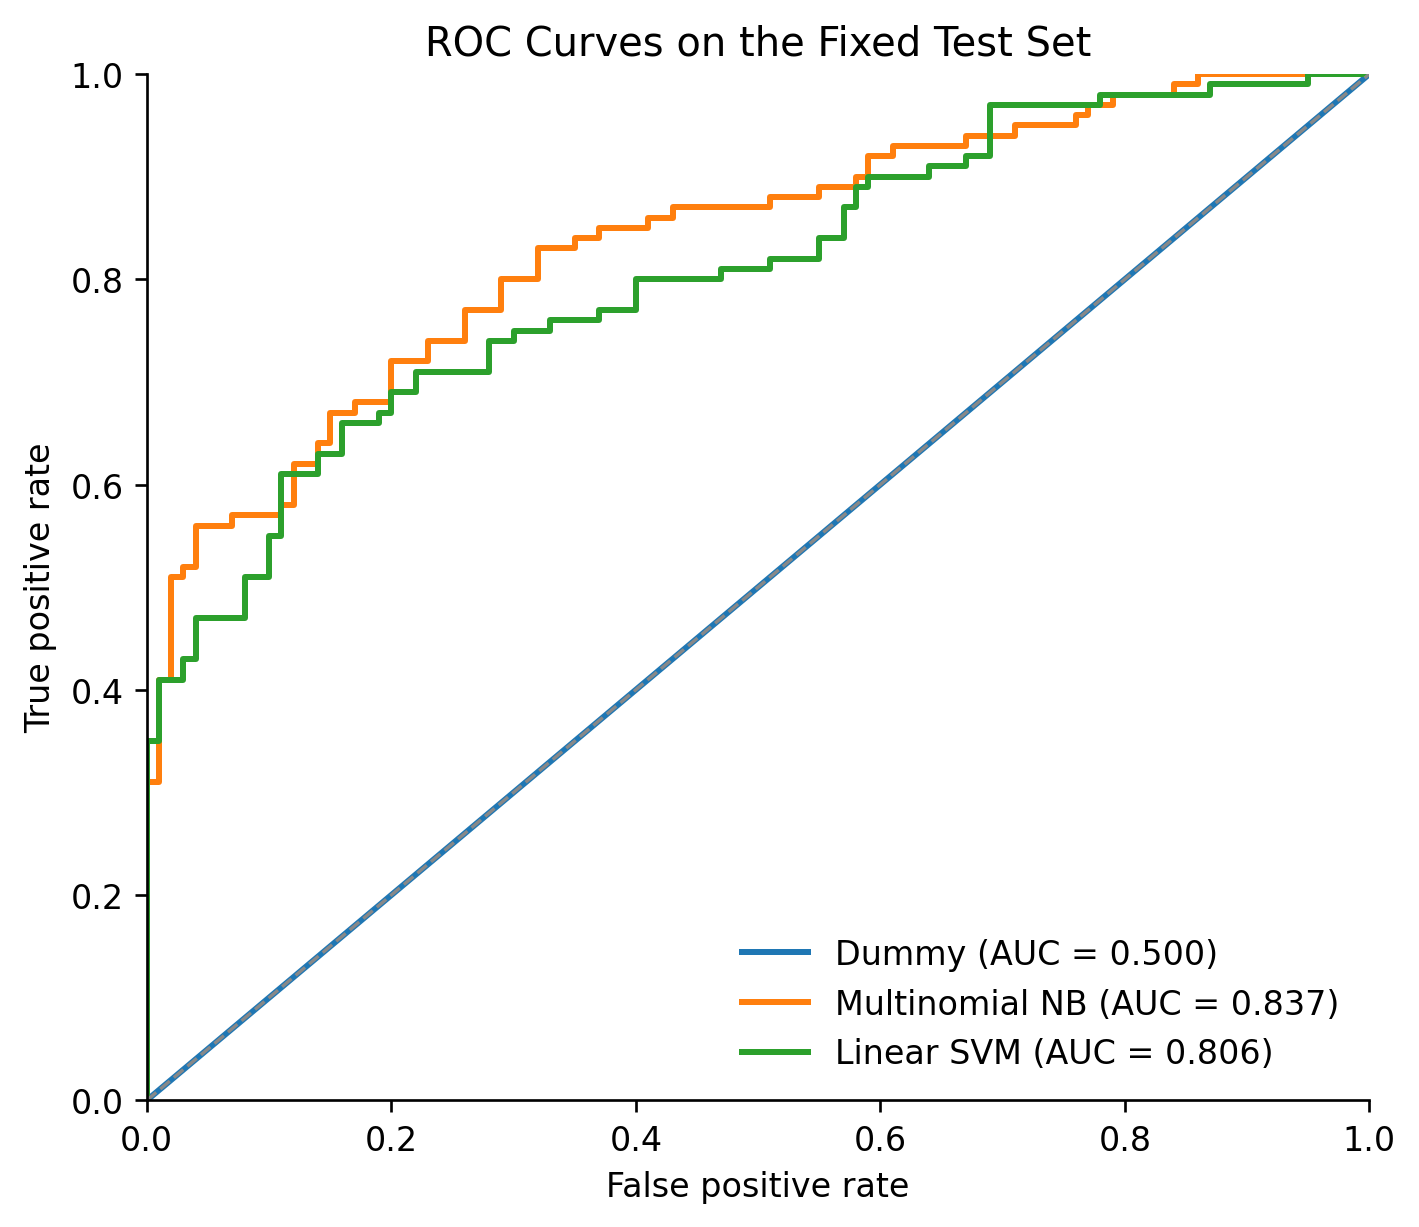
\includegraphics[width=\columnwidth]{../results/figures/final_roc_curves.png}
  \caption{ROC curves of all three models on the fixed test partition. The
  diagonal is the random-classification baseline. The legend reports the
  area under each curve.}
  \label{fig:final-roc}
\end{figure}

As shown in Figure~\ref{fig:final-roc}, NB achieved stronger ranking quality
than the locked SVM on this test set (AUC 0.837 versus 0.806). The curves still
cross at some operating points, so deployment choices should consider the
desired precision--recall trade-off rather than AUC alone.

\paragraph{Interpretation of learned weights.}
The strongest positive NB log-odds terms include \emph{great},
\emph{delicious}, \emph{fantastic} and \emph{awesome}; the strongest negative
terms include \emph{terrible}, \emph{bad}, \emph{slow} and the truncated token
\emph{wasn}. The SVM assigns large negative weights to \emph{not}, \emph{wasn}
and \emph{don}. These weights reflect corpus frequency and the tokenizer's
treatment of contractions: \emph{isn't} becomes \emph{isn} plus a discarded
single-character fragment, so the model cannot reliably interpret contracted
negation. High weights are explanatory cues, not causal evidence about what
makes a review positive or negative.

\section{Error Analysis}
\label{sec:error-analysis}

We inspected every test review that was misclassified and assigned one
descriptive category by a fixed priority: mixed positive and negative cue
words, negation or contraction, contrast or qualification, short review
(at most six word tokens), and other. These labels organize manual review;
they are not manually validated semantic annotations and do not imply
causation. A review may carry several flags, but it contributes to only one
primary category. An error is marked high-confidence when its score lies at
least at the model's own upper quartile of distance from the neutral score.

\begin{table}[t]
  \caption{Descriptive error counts on the same 200-review test partition.
  FP = negative review predicted positive; FN = positive review predicted
  negative. The two boolean flag columns overlap with the category counts.}
  \label{tab:error-summary}
  \centering
  \begin{tabular}{lrrrrrrrr}
    \hline
    Model & Errors & FP & FN & High conf. & Negation & Contrast & Short & Other \\
    \hline
    Multinomial NB & 50 & 22 & 28 & 2 & 10 & 2 & 16 & 23 \\
    Linear SVM & 49 & 18 & 31 & 3 & 12 & 3 & 11 & 24 \\
    \hline
  \end{tabular}
\end{table}

NB made 50 errors (25.0\%) and SVM made 49 (24.5\%). Most errors are not
extreme-confidence mistakes: only two NB errors and three SVM errors lie in
the upper quartile of their score margins. This suggests that the decision
boundary, rather than a few confidently wrong reviews, drives the observed
error rate. Sixteen NB errors were short reviews of at most six word tokens;
such texts provide little lexical evidence for either class. Ten NB errors
contained an explicit negation token, and two contained a contrast marker.
No NB error contained both a positive and a negative cue word from our small
heuristic lexicon, so the mixed-cue category has zero cases in the saved error
summary; this reflects the limited coverage of the lexicon, not the absence of
mixed sentiment in natural language.

\paragraph{Representative cases.}
Review IDs in the local audit file refer to the fixed cleaned corpus. For
example, NB misclassified review 396 and review 109 as negative with scores
0.234 and 0.226 respectively; the first was flagged for negation and the
second for short length. Review 21 was misclassified as positive with a score
of 0.550 and only three word tokens. These IDs let the group locate cases in
the local error file without redistributing full review text. We deliberately
do not paste the original comments into the report because the data license
does not grant redistribution rights.

\begin{figure}[t]
  \centering
  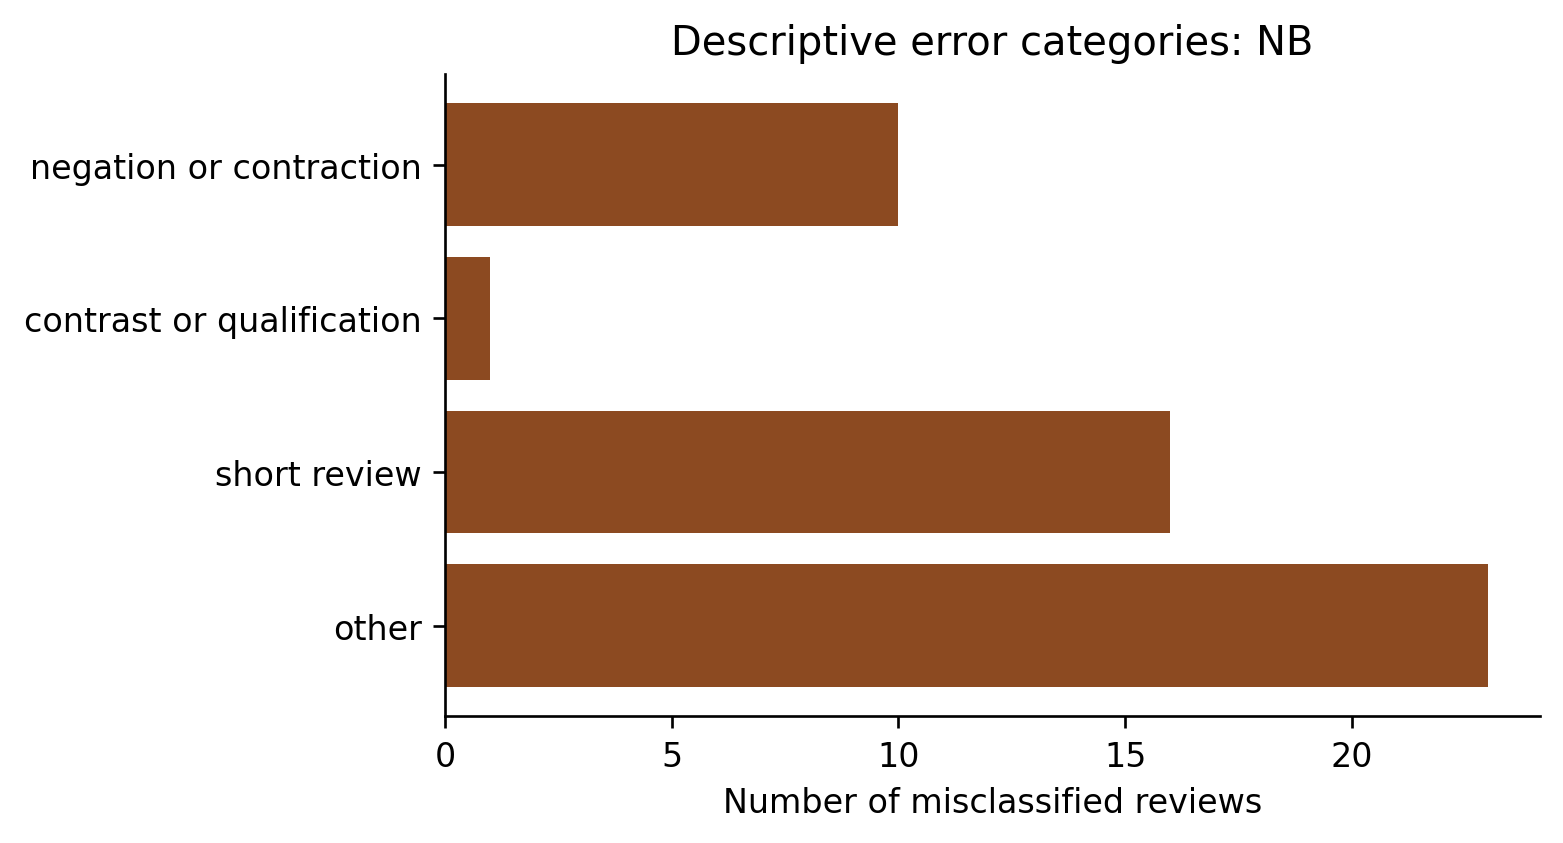
\includegraphics[width=\columnwidth]{../results/figures/final_error_categories.png}
  \caption{Primary descriptive error categories for the highest-F1 model on
  the test partition. Counts are produced by the fixed heuristic priority
  described above and are not causal labels.}
  \label{fig:error-categories}
\end{figure}

\section{Discussion}
\label{sec:discussion}

The experiment answers the three model questions in a limited but reproducible
way. Linear SVM did not outperform Multinomial NB on the fixed test sample: NB
was better in accuracy, recall, positive-class F1 and ROC-AUC, whereas SVM was
better in precision. Word unigrams were already selected by Member 3's
training-only comparison; bigrams did not improve the prespecified F1 and are
not re-tested here. The most discriminative terms are intuitive sentiment
words, but contraction handling and the absence of punctuation features
constrain interpretation.

Several limitations apply. The corpus contains 996 distinct short snippets,
so a 200-review test set gives imprecise estimates; small metric gaps should
not be treated as significant. The majority-class baseline reaches F1 0.667
only because it always predicts the positive class, which gives perfect recall
and no practical discrimination. Error categories rely on a small keyword
heuristic rather than human annotation, and the NB log-odds and SVM weights
are associations learned from this corpus. Finally, all reported numbers
use Member 4's locked $C=0.1$ SVM setting. Every table, figure and number in
this section is generated by
\texttt{restaurant\_sentiment.final\_evaluation} and recorded in
\texttt{results/tables/final\_evaluation.json}.
